\documentclass{article}

\usepackage[utf8]{inputenc}
\usepackage[francais]{babel}
\usepackage{amsmath}
\usepackage{amssymb}
\usepackage{fancyhdr}
\pagestyle{fancy}
\usepackage{graphicx}
\usepackage{placeins}
\usepackage{minted}


\lhead{Coralie Saysset - Romain Gerard}
\chead{}
\rhead{B3301}


\begin{document}

\begin{center} 
\Huge{Références croisées \\ Spécification et Conception}
\end{center}



%-----------------------------------------------------------------------------------------------------------------------------------%
%	Spécification compléte
%-----------------------------------------------------------------------------------------------------------------------------------%
\begin{section}{Spécification complète}


  \begin{subsection}{Définitions}

    \begin{itemize}

      \item \textbf{mot} : Suite de caractères se terminant par un délimiteur.

      \item \textbf{ligne} : Suite de mots terminée par un retour chariot

      \item \textbf{Identificateur} : Mot sensible à la casse composé uniquement de caractères alphanumériques et du caractère `\_`. 
				      Les commentaires ou chaines litérales ne peuvent contenir d'identifcateurs

      \item \textbf{Délimiteur} : Un caractère représentant une séparation entre deux mots (Ex: une virgule, un espace, un point, ...) 

      \item \textbf{Référence croisée} : Fait de rechercher un identificateur dans un ou plusieurs fichiers sources pour déterminer sa localisation
    \end{itemize}

  \end{subsection}


  \begin{subsection}{Description du programme}
    Le but du programme est de permettre de retrouver rapidement l'emplacement d'identifcateurs dans une collection de fichiers.
    On cherche à connaitre dans quel(s) fichier(s) et à quelle(s) ligne(s) les identifcateurs apparaissent.
    
    Dans le cas où un identifacteur apparaitrait plusieurs fois sur une même ligne, nous avons pris la décision d'afficher
    la ligne concernée autant de fois qu'il y a d'occurences. En effet, un identificateur est un mot clé significatif pour l'utilisateur.
    Nous pouvons donc nous attendre à ce qu'il n'apparaisse que peu sur la même ligne.
    
    Ex: Pour le code ci-dessous présent dans le fichier ``test.cpp'' et avec comme identifacteur la lettre i 
    
    \begin{minted}{cpp}
      for( int i = 0; i < 42; i++ );
    \end{minted}
    Le programme produira la sortie suivante : 

    i$\xrightarrow{}$test.cpp$\bullet$1$\bullet$1$\bullet$1$\downarrow$ \\
    
    Par defaut les identificateurs sont les mots clefs utilisés par le langage C++. Il est cependant possible de spécifier
    un fichier en argument du programme pour définir précisement quelles seront les identifcateurs recherchés par la référence
    croisée. Le fichier d'identifacteurs ne devra contenir qu'un seul identifacteur valide par ligne, le premier mot de la ligne sera choisi comme tel. Le programme présuposera que
    le fichier fourni en argument respecte ce formalisme.
    
    Le programme disposera également de la fonctionnalité permettant d'exclure une liste d'identifacteurs.
    
  \end{subsection}

  
  \newpage
  \begin{subsection}{Spécifications des options}
    \begin{center}
      \textbf{$tp\_stl\ [-e]\ [-k fichier\_mot\_clef]\ [nomfichier]+$}
    \end{center}

    \begin{itemize}
      \item[] \textbf{-e} : Permet d'inverser le comportement par défaut du programme. Exclut de la référence croisée tous les mots clefs du C++
      
      \item[] \textbf{-k fichier\_mot\_clef} : Permet de spécifier au programme une liste d'identifacateurs à rechercher par la référence croisée

      \item[] \textbf{nomfichier} : Chemin vers un ou plusieurs fichiers où rechercher les identifacateurs
    \end{itemize}

  \end{subsection}

\end{section}



%-----------------------------------------------------------------------------------------------------------------------------------%
%	Tests fonctionnel
%-----------------------------------------------------------------------------------------------------------------------------------%
\begin{section}{Tests fonctionnels}

 \begin{subsection}{Méthodologie}
  
    Nous sommes parti du principe que le programme doit produire la même sortie écran (et donc par extension les mêmes données stockées en interne)
    si il est lancé deux fois sur la même collection de fichiers et avec les mêmes arguments.

    En partant de ce principe nous avons réaliser les tests de la façon suivante : 

    \begin{enumerate}
      \item Lancer le programme sur une collection de fichier
      \item Verifier que la sortie est correcte et respecte les spécifications
      \item Relancer le programme dans le même contexte qu'en 1, trier la sortie et rediriger le flux de sortie dans un fichier témoin
    \end{enumerate}

    Pour automatiser les tests nous avons écrit un script bash qui suit les étapes suivantes pour chaque test :
  
    \begin{enumerate}
      \item Lancer le programme dans le même contexte que lors de la réalisation du fichier témoin, trier la sortie et rediriger la sortie vers un fichier résultat
      \item Faire le hash md5 du fichier résultat et du fichier témoin
      \item Comparer les deux hash md5
      \item Si les hashs diffèrent c'est que le programme ne possède pas les mêmes données en interne et donc le test échoue
      \item Si les hashs sont égaux c'est que le programme possède les mêmes données et donc le test réussi
    \end{enumerate}

 \end{subsection}




 \begin{subsection}{Critique de la méthode}
    \begin{paragraph}{Avantages :}
      Avec cette méthode de réalisation des tests on s'abstrait de la représentation interne des données. On vérifie uniquement
      que le programme délivre correctement à l'utilisateur les informations voulues. Ainsi tout changement dans la structure de
      données interne n'affectera pas les tests tant que le programme délivre les memes informations à l'utilisateur.
      
      De plus la réalisation d'un test supplémentaire se fait facilement et ne prend pas beaucoup de temps par rapport à une analyse
      compléte de la structure de données interne.
      
      Nous gardons une sauvegarde du flux de sortie lors d'un état fonctionnel de l'application, de ce fait, le développeur peut 
      comparer visuellement les deux sorties pour trouver plus facilement les éléments divergeants. D'où un gain de temps lors du débuggage 
    \end{paragraph}

    \begin{paragraph}{Inconvénients :}
      Avec cette méthode, le formatage des informations à l'utilisateur devient un élément critique. Tout changement dans l'affichage des résultats causera
      inevitablement l'échec de tous les tests. Toutefois, il peut être facile de créer un script bash permettant de regénérer les fichiers témoins
      si le développeur est sur des changements qu'il a effectués.
      
      Si un fichier témoin venait à être corrompu cela entrainerait l'échec du test le mettant en jeu.
    \end{paragraph}
 \end{subsection}

  \newpage
  
  \begin{subsection}{Test \no 1}
    \begin{paragraph}{Descriptif :}
      Le test \no 1 réalise le premier exemple donné par le sujet.\\ Les fichiers analysés sont : 
      
      \begin{listing}[h!]
      \centering{file1.cpp}
      \begin{minted}[linenos,
		     gobble=2]{cpp}
	  // affiche le message "Hello world"
	  int main() {
	      cout <<"Hello world"<<endl;
	      cout<<endl;
	      return 0;
	  }
      \end{minted}
      \end{listing}
      
      \begin{listing}[h!]
      \centering{file1.h}
	\begin{minted}[linenos,gobble=2]{cpp}
	   int main();
	\end{minted}
      \end{listing}
      
        \begin{listing}[h!]
        \centering{key1.txt}
	\begin{minted}[linenos,gobble=2]{cpp}
	   int
	   world
	   template
	\end{minted}
      \end{listing}
      
    \end{paragraph}
    
    \begin{paragraph}{Résultat attendu :} 
      Nous lançons le programme avec le contexte suivant :  
       \begin{center}
	\textbf{$tp\_stl\ -e\ -k\ key1.txt\ file1.cpp\ file1.h$}
      \end{center}
      
      Nous devons obtenir le résultat ci-dessous après avoir trié la sortie : 
      \begin{listing}[h!]
          \centering{file1.res}
      \begin{minted}[linenos,
		     gobble=2]{pascal}
	  cout	file1.cpp 3 4	
	  endl	file1.cpp 3 4	
	  main	file1.cpp 2	file1.h 1	
	  return	file1.cpp 5	
      \end{minted}
  
      \end{listing}
    \end{paragraph}

 \end{subsection}
     
   \newpage 
       
  \begin{subsection}{Test \no 2}
  
    \begin{paragraph}{Descriptif :}
	Le test \no 2 réalise le deuxième exemple donné par le sujet.\\ Les fichiers analysés sont : 
      
      \begin{listing}[h!]
      \centering{file2.cpp}
      \begin{minted}[linenos,
		     gobble=2]{cpp}
	  // affiche le message "Hello world"
	  int main() {
	      cout <<"Hello world"<<endl;
	      cout<<endl;
	      return 0;
	  }
      \end{minted}
      \end{listing}
      
      \begin{listing}[h!]
      \centering{file2.h}
	\begin{minted}[linenos,gobble=2]{cpp}
	   int main();
	\end{minted}
      \end{listing}
      
        \begin{listing}[h!]
        \centering{key2.txt}
	\begin{minted}[linenos,gobble=2]{cpp}
	   int
	   world
	   template
	\end{minted}
      \end{listing}
      
    \end{paragraph}
	   
    \begin{paragraph}{Résultat attendu :}
       Nous lançons le programme avec le contexte suivant après avoir trié la sortie :  
       \begin{center}
	\textbf{$tp\_stl\ -k\ key2.txt\ file2.cpp\ file2.h$}
      \end{center}
      
      Nous devons obtenir le résultat ci-dessous : 
      \begin{listing}[h!]
          \centering{file2.res}
      \begin{minted}[linenos,
		     gobble=2]{pascal}
	  int	file2.cpp 2	file2.h 1	
      \end{minted}
  
      \end{listing}
    \end{paragraph}

  \end{subsection}

   \newpage 
  
  \begin{subsection}{Test \no 3}
    
    \begin{paragraph}{Descriptif :}
	Le test \no 3 réalise le test sur le fichier main de notre programme.\\ Les fichiers analysés sont : 
      
      \begin{minted}[linenos,
		     gobble=2]{cpp}
	    //============================================================================
	    // Name        : Ref_croisee.cpp
	    // Author      :
	    // Version     :
	    // Copyright   : Your copyright notice
	    // Description : Hello World in C++, Ansi-style
	    //============================================================================

	    #include <iostream>
	    #include <vector>

	    #include "CmdLine/cmdLine.hpp"
	    #include "References/Referenceur.hpp"
	    #include "References/References.hpp"

	    using namespace std;
	    using namespace Reference_croisee;

	    int main( int argc, char** argv )
	    {/*{{{*/

		CmdLine::Arguments args;
		CmdLine::Parser parser( "Permet de referencer des mots clefs a travers des fichiers" );
		parser.addOption( "exclude,e",  "Inverse le fonctionnement du programme" );
		parser.addOption( "keyword,k",  "Specifie la liste des mots clefs a utiliser", true );

		try {
		    parser.parse( argc, argv, args );

		} catch( exception& e ) {
		    cout << "Une erreur c'est produit durant la recuperation de la ligne de commande : "
			 << endl << e.what() << endl;
		}

		//----------------------------------------------------------------------
		//  On charge les fichiers a referencer
		//----------------------------------------------------------------------
		vector<string> ficsReferencer;

		if( args.count( "__args__" ) ) {
		    ficsReferencer = args.get<vector<string> >( "__args__" );

		} else {
		    cerr << "Aucun fichier a referencer !" << endl;
		    return 1;
		}

		//----------------------------------------------------------------------
		//  On charge les mots clefs si ils sont fournis
		//----------------------------------------------------------------------
		string fichierMotClef;

		if( args.count( "keyword" ) ) {
		    fichierMotClef = args.get<string>( "keyword" );
		}

		//----------------------------------------------------------------------
		//  L'etat dans lequel mettre le programme
		//----------------------------------------------------------------------
		bool mode( args.count( "exclude" ) );


		References refs;

		//----------------------------------------------------------------------
		//  On effectue la reference croisee
		//----------------------------------------------------------------------
		try {
		    Referenceur referenceur( fichierMotClef, mode );
		    referenceur.referencer( ficsReferencer, refs );

		} catch( exception& e ) {
		    cerr << "Une erreur est survenue durant la reference croisee : " << endl;
		    cerr << e.what() << endl;
		}


		//----------------------------------------------------------------------
		//  On affiche les resultats
		//----------------------------------------------------------------------
		refs.display( cout );

		return 0;
	    }/*}}}*/
      \end{minted}
      
    \end{paragraph}
    
    \newpage 
    
    \begin{paragraph}{Résultat attendu :}
       Nous lançons le programme avec le contexte suivant :  
       \begin{center}
	\textbf{$tp\_stl\ file3.cpp$}
      \end{center}
      
      Nous devons obtenir le résultat ci-dessous après avoir trié la sortie: 
      \begin{listing}[h!]
          \centering{file3.res}
      \begin{minted}[linenos,
		     gobble=2]{pascal}
	  bool	file3.cpp 60	
	  catch	file3.cpp 30 72	
	  char	file3.cpp 19	
	  cout	file3.cpp 31 81	
	  else	file3.cpp 43	
	  if	file3.cpp 40 53	
	  int	file3.cpp 19 19	
	  namespace	file3.cpp 16 17	
	  return	file3.cpp 45 83	
	  true	file3.cpp 25	
	  try	file3.cpp 27 68	
	  using	file3.cpp 16 17		
      \end{minted}
  
      \end{listing}
    \end{paragraph}
    
    
  \end{subsection}

  \newpage

  \begin{subsection}{Test \no 4}
    \begin{paragraph}{Descriptif :}
      Le fichier à analyser est le même que dans le test précédent, seul le contexte d'execution change.
    \end{paragraph}
    
\begin{paragraph}{Résultat attendu :}
       Nous lançons le programme avec le contexte suivant :  
       \begin{center}
	\textbf{$tp\_stl\ file4.cpp$}
      \end{center}
      
      Nous devons obtenir le résultat ci-dessous après avoir trié la sortie: 
      \begin{listing}[h!]
          \centering{file4.res}
      \begin{minted}[linenos,
		     gobble=2]{cpp}
	  addOption	file4.cpp 24 25	
	  argc	file4.cpp 19 28	
	  args	file4.cpp 22 28 40 41 53 54 60	
	  Arguments	file4.cpp 22	
	  argv	file4.cpp 19 28	
	  cerr	file4.cpp 44 73 74	
	  CmdLine	file4.cpp 22 23	
	  count	file4.cpp 40 53 60	
	  display	file4.cpp 81	
	  e	file4.cpp 30 32 72 74	
	  endl	file4.cpp 31 32 44 73 74	
	  exception	file4.cpp 30 72	
	  fichierMotClef	file4.cpp 51 54 69	
	  ficsReferencer	file4.cpp 38 41 70	
	  get	file4.cpp 41 54	
	  main	file4.cpp 19	
	  mode	file4.cpp 60 69	
	  parse	file4.cpp 28	
	  Parser	file4.cpp 23	
	  parser	file4.cpp 23 24 25 28	
	  Reference_croisee	file4.cpp 17	
	  referencer	file4.cpp 70	
	  References	file4.cpp 63	
	  Referenceur	file4.cpp 69	
	  referenceur	file4.cpp 69 70	
	  refs	file4.cpp 63 70 81	
	  std	file4.cpp 16	
	  string	file4.cpp 38 41 51 54	
	  vector	file4.cpp 38 41	
	  what	file4.cpp 32 74	
      \end{minted}
  
      \end{listing}
    \end{paragraph}
  \end{subsection}

\end{section}


%-----------------------------------------------------------------------------------------------------------------------------------%
%	Architecture générale
%-----------------------------------------------------------------------------------------------------------------------------------%
\begin{section}{Architecture générale}

  \begin{subsection}{Diagramme de classe du module CmdLine}
    \begin{figure}[htp]
      \begin{center}
	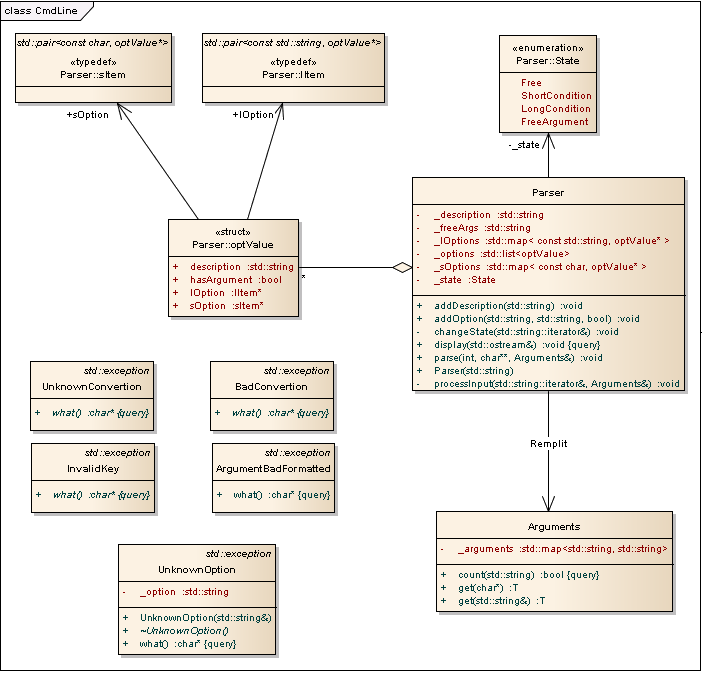
\includegraphics[scale=0.5]{./diagrammeClasse_cmdLine.png}
	% diagrammeClasse.png: 1690x684 pixel, 72dpi, 59.61x24.13 cm, bb=0 0 1690 684
      \end{center}
    \end{figure}
    \FloatBarrier
      Ce diagramme présente les différentes classes présentes pour extraire les informations de la ligne de commande de façon générique.
      
      La classe ``Parser'' s'occupe d'extraire les informations de la ligne de commande en vérifiant que les options entrées par l'utilisateur
      respectent celles définies par le développeur du programme. Au fur et à mesure de l'extraction des données, la classe ``Parser'' remplit
      un objet de la classe ``Arguments''. La classe ``Arguments'' sert de conteneur et permet de convertir les options vers des types déterminés
      à la compilation. Ne sachant pas comment représenter des méthodes génériques en UML, j'ai défini le type de retour des fonctions membres
      ``get'' comme étant T. Le module possède ses propres exceptions pour remonter les cas d'erreurs possibles.
   \end{subsection}
   
   \begin{subsection}{Diagramme de classe du module Reference\_croisée}
    \begin{figure}[!ht]
      \begin{center}
	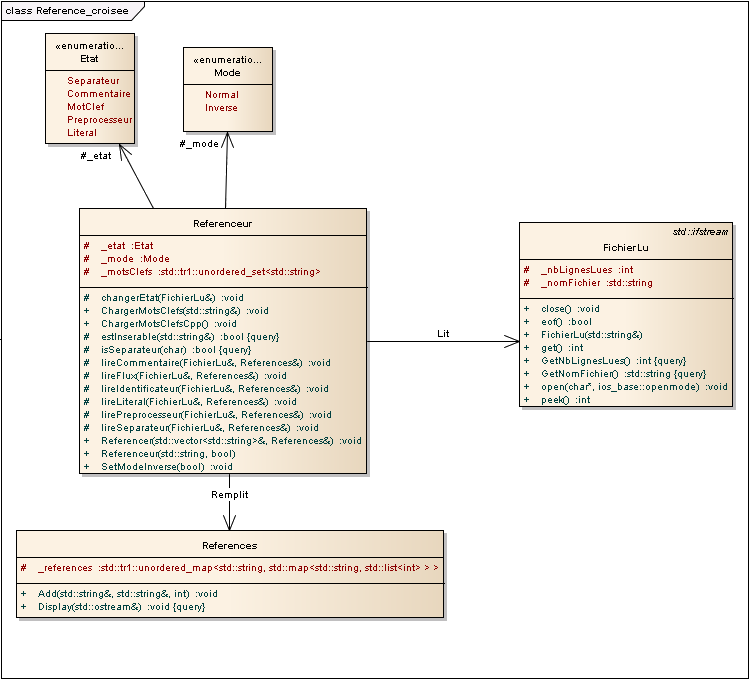
\includegraphics[scale=0.5]{./diagrammeClasse_reference.png}
	% diagrammeClasse.png: 1690x684 pixel, 72dpi, 59.61x24.13 cm, bb=0 0 1690 684
      \end{center}
    \end{figure}
    \FloatBarrier
     Ce diagramme présente les différentes classes utilisées pour extraire les identifacateurs d'un fichier source C++.
      Un objet de la classe ``FichierLu'' permet de lire un fichier stocké sur le disque, tout en fournissant le nombre de lignes déjà 
      lues ainsi que le nom du fichier ouvert. 
      
      Un ``Referenceur'' se sert d'un ``FichierLu'' pour lire les fichiers sources et en extraire les identifacateurs.
      Une collection de ``References'' permet de stocker les identifacteurs qui sont des mots clefs.
   \end{subsection}
   
   \newpage
    \begin{subsection}{Diagramme de classe du module principal}
    \begin{figure}[!ht]
      \begin{center}
	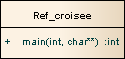
\includegraphics[scale=0.5]{./diagrammeClasse_main.png}
	% diagrammeClasse.png: 1690x684 pixel, 72dpi, 59.61x24.13 cm, bb=0 0 1690 684
      \end{center}
    \end{figure}
    \FloatBarrier
    Le module principal permet d'orchestrer les deux modules précédents pour que le programme ait le comportement attendu.
   \end{subsection}

\end{section}


%-----------------------------------------------------------------------------------------------------------------------------------%
%	Algorithmes principaux
%-----------------------------------------------------------------------------------------------------------------------------------%
\begin{section}{Algorithmes principaux}

  \begin{subsection}{Parseur pour la ligne de commandes}
  Pour extraire les informations de la ligne de commande nous utilisons un automate avec un nombre d'états fini.
  
  \begin{paragraph}{Description des états :}
    \begin{itemize}
      \item \textbf{Free} : Lorsque l'automate rencontre quelque chose qui n'est pas un argument ou une option \\Exemple: un caractère séparateur comme un espace
      \item \textbf{ShortCondition} : Lorsque l'automate rencontre une option courte \\Exemple: -e ou -k
      \item \textbf{LongCondition} : Lorsque l'automate rencontre une option longue \\Exemple: --exclude ou --keyword
      \item \textbf{FreeArgument} : Lorsque l'automate rencontre un argument rataché à aucune option\\Exemple: le nom d'un fichier à analyser\\
    \end{itemize}
  \end{paragraph}
  
  Une action est déclenché en fonction de l'état de l'automate. L'action extrait, analyse et stocke l'argument de la ligne de commande s'il est valide, sinon une exception est levé.
  \end{subsection}

  \begin{subsection}{Parseur pour les fichiers C++}
  Pour extraire les informations de la ligne de commande nous utilisons ici aussi un automate avec un nombre fini d'états.
  
  \begin{paragraph}{Description des états :}
   \begin{itemize}
    \item \textbf{Separateur} : Lorsque que l'automate rencontre un caractère séparant deux identifacteur\\Exemple: Tout caractère non alphanumériques, le tiret du bas non inclus
    \item \textbf{Commentaire} : Lorsque l'automate rencontre un commentaire sur une seule ligne ou multiligne \\Exemple: /* Ceci est un commentaire */
    \item \textbf{MotClef} : Lorsque l'automate rencontre un identifacteur qui peut être un mot clef potentiel \\Exemple: cout
    \item \textbf{Preprocesseur} : Lorsque l'automate rencontre une instruction preprocesseur \\Exemple: \#include $<$iostream$>$
    \item \textbf{Literal} : Lorsque l'automate rencontre une chaine de caractères ou un caractère\\Exemple: ``Bonjour''\\
   \end{itemize}
  \end{paragraph}
  
  Chaque état déclenche une action propre qui a pour tâche d'avancer dans le fichier tout en extrayant les identifacteurs qui sont des mots clefs.
  \end{subsection}

\end{section}



%-----------------------------------------------------------------------------------------------------------------------------------%
%	Structures de données
%-----------------------------------------------------------------------------------------------------------------------------------%
\begin{section}{Analyse critique des structures de données}


  \begin{subsection}{Structure des identificateurs}
\begin {paragraph}{Analyse des besoins}
Les identificateurs sont lus dans un ou plusieurs fichiers passés en parametre. Il faut tout d'abord prendre en considération
deux choses: d'abord la présence de doublon parmi les identificateurs, ce qui n'est pas interdit à l'utilisateur. Leur existence
entraine un surcout d'opération soit lors de test à la création pour l'empecher soit plus tard au traitement. Ensuite l'option
\textbf{-e} permet de soustraire à la liste d'identificateur passée en parametre la liste des mots clés du C++. La structure
 de données choisie pour les identificateurs devra comparer ces deux listes de manière appropriée.


\end paragraph
\end {paragraph}

  \end{subsection}

  \begin{subsection}{Structure des occurences}
\begin{paragraph}{Analyse des besoins}
Si le choix d'une bonne structure pour les identifacateurs est important, pour les occurences il est essentiel pour le 
fonctionnement du programme. En effet chaque idientificateurs peut être trouvés de nombreuses fois dans un documents. Il peut 
y avoir de très grands nombres d'occurences provennant de plusieurs fichiers alors que les identificateurs ne seront contenus
que dans un seul fichier passé en parametre. Par consequent le programme devra être optimisé avant tout pour la manipulation
(acces, insertion, suppression) d'occurences que d'identifacateurs qu'il utilisera moins.
\end{paragraph}

\begin{paragraph}
 Le programme va être amené à rencontrer et traîter de nombreuses occurences. Dans un soucis de réutilisabilité, on considère
que l'utilisateur pourra en plus de voir apparaître les occurences sur la console, vouloir récupérer une structure de donnée
localisant les occurences. Par conséquent nous avons choisi de séparer la fonction pemettant de trouver les occurences et de
les enregistrer de celle permettant d'afficher celles trouvées. On choisira donc de favoriser l'insertion d'élément par
rapport à l'acces, ce qui veut dire que nous favoriserons le traitement par rapport à l'affichage.

\end{paragraph}


  \end{subsection}

\end{section}

\end{document}
